\subsection{External Interface Requirements}
\subsubsection{User Interfaces}
\subsubsection{Hardware Interfaces}
The Students\&Companies (S\&C) platform is a web-based application, so it does not require any specific hardware interface. It is accessible via computers, smartphones, or any other device with a web browser and an internet connection.
\subsubsection{Software Interfaces}
\begin{itemize}
    \item \textbf{Recommendation Engine API} To provide internship recommendations to students based on their profiles, skills, and previous interactions.
    \item \textbf{Email Notification Service} To send notifications to students and companies about internship opportunities, application statuses, and important deadlines.
\end{itemize}
\subsubsection{Communication Interfaces}
The platform requires an active internet connection to allow users to interact with it. Communication between users within the platform is done via messaging and notification systems. Students and companies can also use the platform to exchange information regarding internships, applications, and interviews.

The platform must be HTTPS compliant to ensure secure communication between users and the platform itself, protecting user data and interactions.




\subsection{Functional Requirements}

\begin{enumerate}[label={[R\arabic*]}]
\item[] \textbf{Sign-Up, Login, and Profile Management}


\item The system should provide authentication so that each action can be correctly associated with a user


\item When a student registers the system generates a profile containing their experience, skills, and education


\item[] \textbf{Internship Publication and Management}


\item The system allows companies to create new internship positions at any time


\item When a company user clicks on “create internship”, the system prompts the company for all the required information and checks its validity before saving


\item When an internship is successfully created, the system generates a work profile containing the required experience and skills for the position

 
\item When and internship is successfully created it should be findable through the search internship feature and allow student applications

\item[] \textbf{Search and Apply for Internships}


\item When a student searches for an internship through the platform, the system accurately processes the student’s search criteria to display related internships


\item When an internship is selected, the system’s user interface summarizes internship information


\item When a student searches for an internship through the platform, the displayed internships  are within the selected filters


\item When a student searches for an internship through the platform, the displayed internships are ordered accordingly to the field specified in student’s criteria

\item The system shall allow students to apply to the displayed internship without adding additional information


\item When the application button is clicked, the system shall save the student information and profile and notify the company

\item[] \textbf{Internship Matching and Recommendation}


\item The system shall provide regular monitoring to all stored profiles from students and internships


\item The system shall attempt to match student profiles with internship profiles


\item In every match found between an internship and a student, the system shall notify both parts about it


\item The matching algorithm used to find recommendations is accurate and can be improved through user feedback

\item[] \textbf{Interview Management and Selection Process}


\item The system allows company users to review any student profile


\item The system allows company users to invite any student to an interview


\item The system notifies the company when there are new student profiles to review (either applied or recommended)


\item When the company user clicks on “invite to interview” over a student, the system prompts the company user to provide possible availability slots for that specific interview

 
\item When the company user creates an interview by providing their availability the system notifies the selected student in less than 6 hours after the interview creation


\item The system allows students to decline the interview they have been invited for

 
\item If the student does not reply to the interview invitation after 48 hours from the sending time, the system declines the interview automatically


\item When a student accepts an interview invite, the system prompts them to select one of the available time slots for having the interview


\item The system does not allow the student to accept an interview invite without selecting one of the available slots the system provides


\item When the interview starting time comes (slot start), the system provides the company user with the questionnaire associated with the internship the interview is for


\item When the interview finishing time comes (slot end), the system prompts the company user for an interview verdict (approve or reject)


\item When the company user rejects the student after an interview, the system notifies the student


\item When the company user approves the student after an interview, the system prompts them to provide the start time and place of the internship


\item The system does not allow the company to approve the student without providing the internship start time and place


\item When a company user approves the student after an interview, the system notifies the student of the start time and place of the internship

\item[] \textbf{Feedback and Complaint Management}

\item When the duration time of an internship has passed since its starting time, the system notifies and prompts both the company user and the student to provide feedback on the internship experience


\item The system will not allow any user to use other features of the platform (besides login and feedback) when they have pending feedback on past internships

 
\item When a user provides feedback on an internship the system notifies its counterpart in the internship about the received feedback


\item The system allows any user to create a complaint about any of their ongoing internships

 
\item When a user creates a complaint the system prompts them to provide a non-empty description of the issue

\end{enumerate}

\subsubsection{Use Cases}
\textbf{UC1: Form Filling} (Table \ref{tab:UC1})
\begin{table}[H]
\centering
\caption{\textbf{UC1: Form Filling}}
\label{tab:UC1}
\resizebox{\textwidth}{!}{%
\begin{tabular}{|c|l|}
\hline
\textbf{Actors}           & user                                                       \\ \hline
\textbf{Entry Condition}   & an empty form is displayed on the user’s screen. the user knows all the required information. \\ \hline
\textbf{Event Flow}        & 1. the user completes the form with the required information \\
                           & 2. the user clicks on the “Submit” button                   \\
                           & 3. S\&C validates the inputted information and stores it in its internal database. \\ \hline
\textbf{Exit Condition}    & the data is correctly stored in the system’s internal database. \\ \hline
\textbf{Exceptions}        & the system detects that some of the provided information is invalid or empty.  \\ & it shows an error to the user and prompts them to correct it. \\ \hline
\end{tabular}
}
\end{table}

\textbf{UC2: Register Student }(Table \ref{tab:UC2})
\begin{table}[H]
\centering
\caption{\textbf{UC2: Register Student}}
\label{tab:UC2}
\begin{tabularx}{\textwidth}{|X|X|}
\hline
\textbf{Actors}           & student                                                   \\ \hline
\textbf{Entry Condition}   & the user has opened the S\&C Website and has all the required information. \\ \hline
\textbf{Event Flow}        & 1. S\&C Website initial page prompts the user to identify  \\
                           & 2. The user presses the “New Account” button             \\
                           & 3. S\&C shows a form to be completed with:               \\
                           & \hspace{1em} a. Email                                      \\
                           & \hspace{1em} b. Password                                   \\
                           & \hspace{1em} c. Full Name                                 \\
                           & \hspace{1em} d. Skills, interests, experience, education… \\
                           & 4. Included use case: form filling                        \\ \hline
\textbf{Exit Condition}    & A student is properly registered and has a valid account. \\ \hline
\textbf{Exceptions}        & none                                                      \\ \hline
\end{tabularx}
\end{table}

\textbf{UC3: Register Company }(Table \ref{tab:UC3})
\begin{table}[H]
\centering
\caption{\textbf{UC3: Register Company}}
\label{tab:UC3}
\begin{tabularx}{\textwidth}{|X|X|}
\hline
\textbf{Actors}           & company employee                                         \\ \hline
\textbf{Entry Condition}   & the company employee has opened the S\&C Website and has all the required information. \\ \hline
\textbf{Event Flow}        & 1. S\&C Website initial page prompts the company employee to identify  \\
                           & 2. The company employee presses the “New Account” button             \\
                           & 3. S\&C shows a form to be completed with:                          \\
                           & \hspace{1em} a. Email                                             \\
                           & \hspace{1em} b. Password                                          \\
                           & \hspace{1em} c. Company Name                                      \\
                           & \hspace{1em} d. Industry                                          \\
                           & 4. Included use case: Form Filling                                 \\ \hline
\textbf{Exit Condition}    & A company is properly registered and has a valid account.        \\ \hline
\textbf{Exceptions}        & none                                                           \\ \hline
\end{tabularx}
\end{table}

\textbf{UC4: User Login }(Table \ref{tab:UC4})
\begin{table}[H]
\centering
\caption{\textbf{UC4: User Login}}
\label{tab:UC4}
\begin{tabularx}{\textwidth}{|X|X|}
\hline
\textbf{Actors}           & user                                                       \\ \hline
\textbf{Entry Condition}   & the user has opened the S\&C Website and knows their credentials. \\ \hline
\textbf{Event Flow}        & 1. S\&C Website initial page prompts the user to identify  \\
                           & 2. The user clicks on the “Log In” button                   \\
                           & 3. S\&C shows a form to be completed with:                  \\
                           & \hspace{1em} a. Email                                        \\
                           & \hspace{1em} b. Password                                     \\
                           & 4. Included use case: Form Filling                           \\ \hline
\textbf{Exit Condition}    & User is logged into the platform.                           \\ \hline
\textbf{Exceptions}        & none                                                        \\ \hline
\end{tabularx}
\end{table}

\textbf{UC5: Search Internship }(Table \ref{tab:UC5})
\begin{table}[H]
\centering
\caption{\textbf{UC5: Search Internship}}
\label{tab:UC5}
\begin{tabularx}{\textwidth}{|X|X|}
\hline
\textbf{Actors}           & student                                                   \\ \hline
\textbf{Entry Condition}   & The student is logged into S\&C platform.                  \\ \hline
\textbf{Event Flow}        & 1. S\&C main page shows a search tab with filters            \\
                           & 2. Student taps the search bar and specifies the relevant information by either keywords or filters (company name, duration, …) \\
                           & 3. S\&C shows a list of matching available internships      \\
                           & 4. Student scrolls through her/his options and compares them as he/she wills \\
                           & 5. Student clicks on a specific internship opportunity      \\
                           & 6. S\&C shows the internship’s details                      \\ \hline
\textbf{Exit Condition}    & Student has performed the search and knows more about the internships he/she can apply to \\ \hline
\textbf{Exceptions}        & There is no matching result for the search. S\&C throws a “no results” page and suggests the user to alter filters. \\ \hline
\end{tabularx}
\end{table}

\textbf{UC6: Apply Internship }(Table \ref{tab:UC6})
\begin{table}[H]
\centering
\caption{\textbf{UC6: Apply Internship}}
\label{tab:UC6}
\begin{tabularx}{\textwidth}{|X|X|}
\hline
\textbf{Actors}           & student                                                   \\ \hline
\textbf{Entry Condition}   & The student is logged into S\&C platform and currently in a specific internship’s main page \\ \hline
\textbf{Event Flow}        & 1. Along with the internship details, the internship offer main page shows an “easy-apply” button \\
                           & 2. The user clicks the button willing to apply for it       \\
                           & 3. S\&C registers their application, shows a page of “Application Successful” and informs the student that he/she is going to receive feedback in 1 month at worst \\ \hline
\textbf{Exit Condition}    & Student has applied successfully to an internship position \\ \hline
\textbf{Exceptions}        & none                                                      \\ \hline
\end{tabularx}
\end{table}



\textbf{UC7: New Recommendation }(Table \ref{tab:UC7})
\begin{table}[H]
\centering
\caption{\textbf{UC7: New Recommendation}}
\label{tab:UC7}
\begin{tabularx}{\textwidth}{|X|X|}
\hline
\textbf{Actors}           & RecommenderSystem                                         \\ \hline
\textbf{Entry Condition}   & There exists at least one student and one internship, both properly registered in the system, it’s the time where the recommender system is scheduled \\ \hline
\textbf{Event Flow}        & 1. RecommenderSystem scans S\&C’s database via API \\
                           & 2. RecommenderSystem outputs a list of recommendations and posts them to S\&C (API call) \\
                           & 3. Included Use case: Send Notification. S\&C receives the recommendations and for each one of them it \\
                           & 4. S\&C sends a notification to the student about the new internship suggestion and a link to apply immediately. \\ \hline
\textbf{Exit Condition}    & The student is aware of a new internship option and is informed about it with an actionable link \\ \hline
\textbf{Exceptions}        & The RecommenderSystem does not generate any valid matches.  \\ \hline
\end{tabularx}
\end{table}

\textbf{UC8: New Internship }(Table \ref{tab:UC8})
\begin{table}[H]
\centering
\caption{\textbf{UC8: New Internship}}
\label{tab:UC8}
\begin{tabularx}{\textwidth}{|X|X|}
\hline
\textbf{Actors}           & company employee                                         \\ \hline
\textbf{Entry Condition}   & The company employee is logged in and knows all the detail about the internship position he/she wants to create \\ \hline
\textbf{Event Flow}        & 1. The company employee clicks on “New Internship Position”  \\
                           & 2. S\&C shows a form to be completed with the relevant information: \\
                           & \hspace{1em} a. Internship Position Name                    \\
                           & \hspace{1em} b. Internship Position Requirements (skills, previous experience…) \\
                           & \hspace{1em} c. Internship Position Description (Project, tasks to be performed) \\
                           & \hspace{1em} d. Internship Position Compensation & Benefits \\
                           & \hspace{1em} e. Internship Position Duration               \\
                           & \hspace{1em} f. Internship Position Customized Questionnaire for Interviews \\
                           & 3. Included Use Case: form filling \\
                           & 4. S\&C saves the new internship position in its internal database, publishes it and informs the company employee that the position has been created successfully \\ \hline
\textbf{Exit Condition}    & A new internship position is created successfully.       \\ \hline
\textbf{Exceptions}        & none                                                      \\ \hline
\end{tabularx}
\end{table}

\textbf{UC9: Cancel Internship }(Table \ref{tab:UC9})
\begin{table}[H]
\centering
\caption{\textbf{UC9: Cancel Internship}}
\label{tab:UC9}
\begin{tabularx}{\textwidth}{|X|X|}
\hline
\textbf{Actors}           & company employee                                         \\ \hline
\textbf{Entry Condition}   & The company employee is logged in and there’s an open internship for the company \\ \hline
\textbf{Event Flow}        & 1. The company employee clicks on “Open Internships”         \\
                           & 2. A list of open internships appear, he/she clicks on the internship he/she wants to cancel \\
                           & 3. He/she clicks on “Cancel Internship”                     \\
                           & 4. S\&C shows a pop-up asking for confirmation, he/she then clicks on confirm \\
                           & 5. S\&C changes the internship state to “cancelled”, stops showing it in the searches nor recommendations, and no longer receives applications. \\ \hline
\textbf{Exit Condition}    & The desired internship position is cancelled.             \\ \hline
\textbf{Exceptions}        & none                                                      \\ \hline
\end{tabularx}
\end{table}

\textbf{UC10: Schedule Interview }(Table \ref{tab:UC10})
\begin{table}[H]
\centering
\caption{\textbf{UC10: Schedule Interview}}
\label{tab:UC10}
\begin{tabularx}{\textwidth}{|X|X|}
\hline
\textbf{Actors}           & company employee, student                                \\ \hline
\textbf{Entry Condition}   & Company employee is interested in scheduling an interview with a student (either recommended or applied). Both actors are properly registered. The company employee is logged into the platform. \\ \hline
\textbf{Event Flow}        & 1. The company employee clicks on “Schedule an Interview” next to a student’s name or in a notification. \\
                           & 2. S\&C prompts her to input her availability for the next week, desired interview duration and position they’re interviewing for if they have more than one opened at the moment (Included Use Case: form filling) \\
                           & 3. S\&C receives the scheduling request and sends an email to the student, inviting them to the first available slot from the ones provided by the company employee (Included Use Case: send notification) \\
                           & 4. The student opens the email and clicks on the Find a Time button \\
                           & 5. (Included Use Case: user login) \\
                           & 6. Student is prompted to select one of the available slots for interview, then to confirm his/her selection \\
                           & 7. S\&C saves the interview in its internal database and notifies the interviewer (Included Use Case: send notification). \\ \hline
\textbf{Exit Condition}    & A new interview is scheduled correctly and stored in the system’s database. \\ \hline
\textbf{Exceptions}        & The student cannot assist in any of the available slots or is not interested. He clicks on the “Decline” button and is redirected to the main page. No interview is created. \\ \hline
\end{tabularx}
\end{table}

\textbf{UC11: Process Interview }(Table \ref{tab:UC11})
\begin{table}[H]
\centering
\caption{\textbf{UC11: Process Interview}}
\label{tab:UC11}
\begin{tabularx}{\textwidth}{|X|X|}
\hline
\textbf{Actors}           & company employee, student                                \\ \hline
\textbf{Entry Condition}   & There’s an interview scheduled between a company employee and a student. Both actors are properly registered, the company employee is logged into the platform. \\ \hline
\textbf{Event Flow}        & 1. The company employee clicks on “Start Interview” \\
                           & 2. S\&C shows the customized questionnaire associated with the internship position the company is interviewing for \\
                           & 3. Included Use Case: form filling \\
                           & 4. The company employee either approves or rejects the candidate when prompted \\
                           & \hspace{1em} a. If he/she approves the candidate, S\&C asks them to provide start date, time and place of the internship (Included Use Case: form filling) \\
                           & 5. S\&C saves the interview verdict and information. \\
                           & 6. S\&C sends a notification to the student with the verdict and, only if approved, the start date, time and place of the internship. \\ \hline
\textbf{Exit Condition}    & The interview is closed with a verdict and stored in the system’s database. \\ \hline
\textbf{Exceptions}        & The student doesn’t show up. In that case, the company employee can click on the “No Show” button in the questionnaire, and the candidate is rejected automatically. \\ \hline
\end{tabularx}
\end{table}

\textbf{UC12: New Complaint }(Table \ref{tab:UC12})
\begin{table}[H]
\centering
\caption{\textbf{UC12: New Complaint}}
\label{tab:UC12}
\begin{tabularx}{\textwidth}{|X|X|}
\hline
\textbf{Actors}           & user                                                       \\ \hline
\textbf{Entry Condition}   & There’s an ongoing internship involving the user. The user is registered and logged into the platform. \\ \hline
\textbf{Event Flow}        & 1. User clicks on “Ongoing Internships” in the website menu and then selects the internship he/she wants to complain about \\
                           & 2. Then, he/she clicks on “Create Complaint” \\
                           & 3. S\&C displays a form prompting the user to provide a detailed description of the problem (Included Use Case: form filling) \\
                           & 4. S\&C saves the complaint in its internal database. \\ \hline
\textbf{Exit Condition}    & A new complaint is stored in the system’s internal database. \\ \hline
\textbf{Exceptions}        & none                                                      \\ \hline
\end{tabularx}
\end{table}


\textbf{UC13: Post Internship Feedback }(Table \ref{tab:UC13})
\begin{table}[H]
\centering
\caption{\textbf{UC13: Post Internship Feedback}}
\label{tab:UC13}
\begin{tabularx}{\textwidth}{|X|X|}
\hline
\textbf{Actors}           & user                                                       \\ \hline
\textbf{Entry Condition}   & There’s a completed internship involving the user. The user is correctly registered. \\ \hline
\textbf{Event Flow}        & 1. User clicks on “Give Feedback” on the email notification he/she received about a completed internship \\
                           & 2. The user is redirected to the S\&C web-app \\
                           & 3. Included Use Case: user login \\
                           & 4. S\&C displays a form prompting the user to provide feedback (Included Use Case: form filling) \\
                           & 5. The user provides ratings and comments about the internship experience \\
                           & 6. S\&C saves the feedback in its internal database and updates the internship status accordingly. \\
                           & 7. S\&C sends a notification to the company, notifying them that feedback has been submitted. \\ \hline
\textbf{Exit Condition}    & The internship feedback is saved and the status is updated. Both the user and the company have been notified. \\ \hline
\textbf{Exceptions}        & If the user doesn’t submit feedback, the process remains pending. S\&C sends a reminder notification to the user to provide feedback within a set time frame (e.g., 3 days). \\ \hline
\end{tabularx}
\end{table}

\clearpage
\subsubsection{Use Case Diagram}

\begin{figure}[H]
\centering
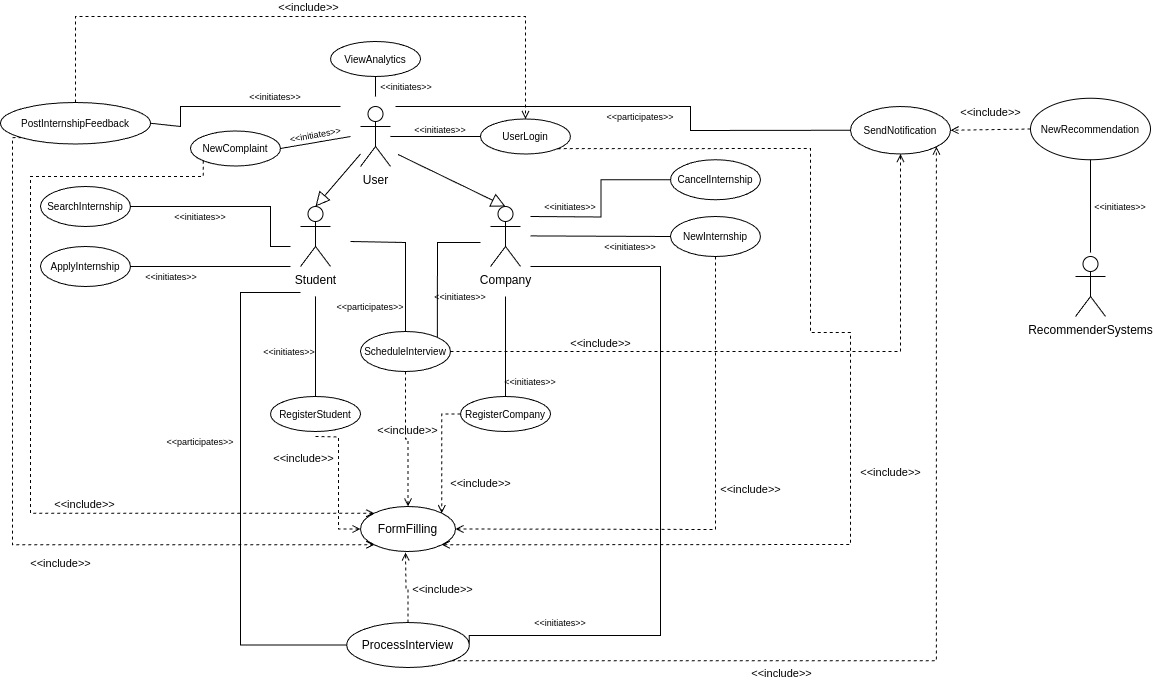
\includegraphics[width=\textwidth]{Images/use_case_diagram.png}
\caption{\label{fig:use-case-diagram} Use Case Diagram}
\end{figure}

\clearpage
\subsubsection{Sequence Diagrams}
We created sequence diagrams for the key use cases: Search Internship, New Recommendation, Matchmaking and Schedule Interview. We believe that through the understanding of these use cases in dept it is possible to shed some light onto the inner workings of the S\&C platform.

\textbf{UC5: Search Internship} (Figure \ref{fig:search_sequence})
\begin{figure}[H]
\centering
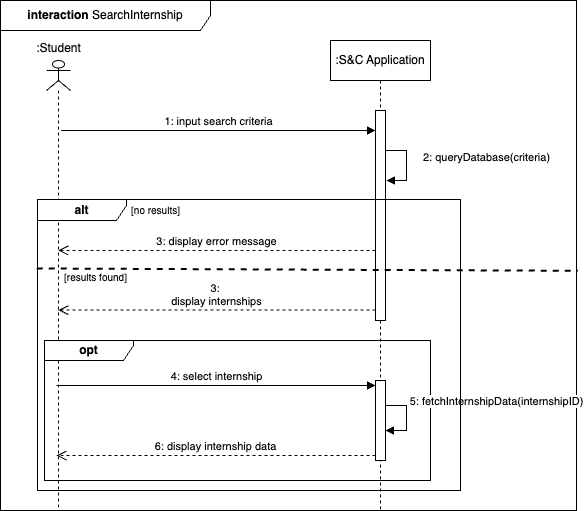
\includegraphics[width=\textwidth]{Images/searchInternship-sequence.png}
\caption{\label{fig:search_sequence} Search Internship Sequence Diagram}
\end{figure}

\textbf{UC7: New Recommendation} (Figure \ref{fig:matchmaking})
\begin{figure}[H]
\centering
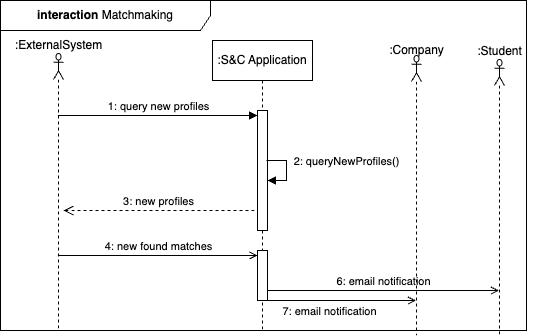
\includegraphics[width=\textwidth]{Images/matchmaking-sequence.png}
\caption{\label{fig:matchmaking} New Recommendation Sequence Diagram}
\end{figure}



\textbf{UC10: Schedule Interview} (Figure \ref{fig:schedule_sequence})
\begin{figure}[H]
\centering
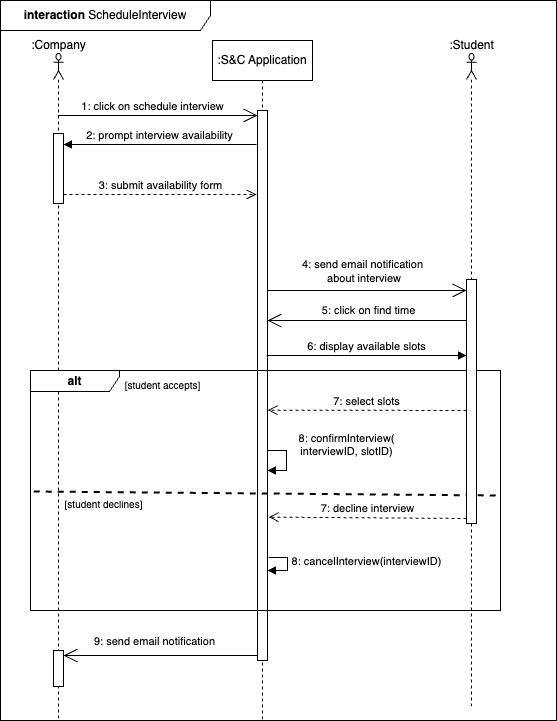
\includegraphics[width=\textwidth]{Images/scheduleInterview-sequence.png}
\caption{\label{fig:schedule_sequence} Schedule Interview Sequence Diagram}
\end{figure}

\textbf{UC11: Process Interview} (Figure \ref{fig:process_sequence})
\begin{figure}[H]
\centering
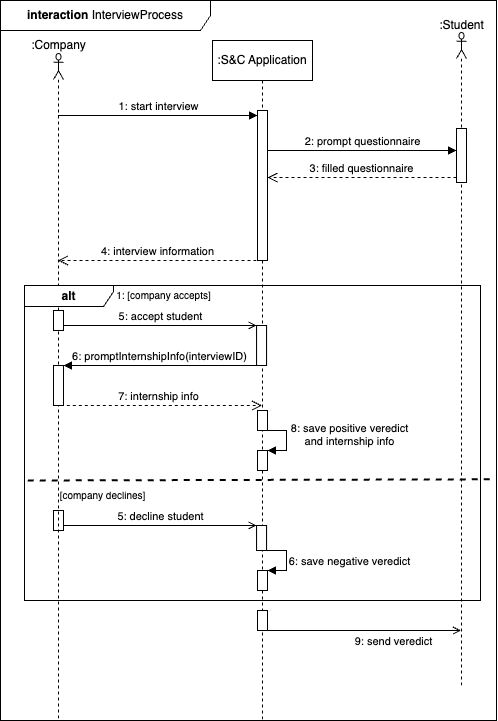
\includegraphics[width=\textwidth]{Images/interviewProcess-sequence.png}
\caption{\label{fig:process_sequence} Process Interview Sequence Diagram}
\end{figure}

\subsubsection{Activity Diagram}
We chose to include this activity diagram because it captures the complete end-to-end selection process on the S\&C platform. It highlights the interactions between the system, a single student, and a single company, illustrating how these parties engage throughout the application, interview, and internship stages.

This diagram emphasizes the interconnectedness of actions and decisions, providing a clear view of how the system facilitates and supports each step. By focusing on this interaction, we aim to provide readers with an intuitive understanding of the process and its flow, making the platform's functionality more transparent and comprehensible.

\begin{figure}[H]
\centering
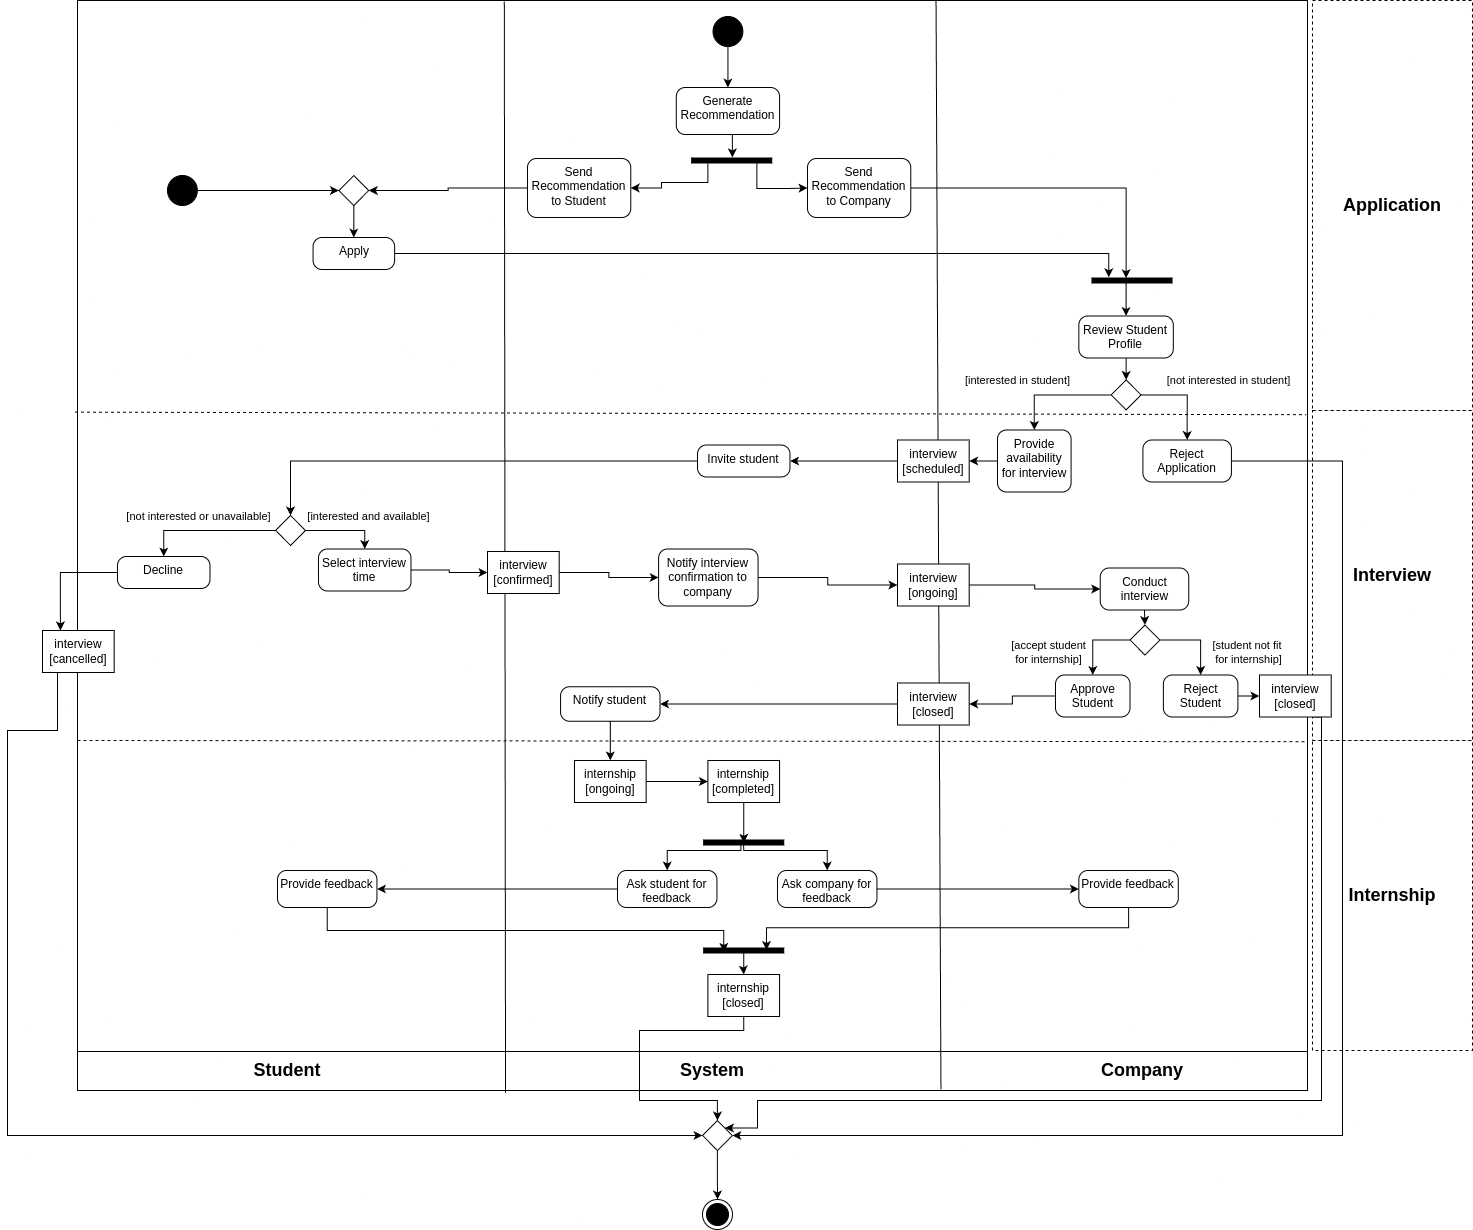
\includegraphics[width=\textwidth]{Images/activity-diagram.png}
\caption{\label{fig:activity_diagram} Activity Diagram}
\end{figure}


\subsubsection{Requirement Mapping}
\textbf{G1: Students are able to look for internships and easily recognize the ones that match their characteristics (skills, interests, experience…)} (Table \ref{tab:g1_Req_mapping})

\begin{table}[H]
\centering
\begin{tabular}{|p{6cm}|p{6cm}|} \hline
\textbf{Requirements} & \textbf{Domain Assumptions} \\
\hline
\begin{tabular}[c]{@{}l@{}}{[}R2{]} When a student registers, the \\ system generates a profile containing \\ their experience, skills, and education.\\ \\ {[}R5{]} When an internship is successfully \\ created, the system generates a work \\ profile containing the required \\ experience and skills for the position.\\ \\ {[}R6{]} When an internship is successfully \\ created, it should be findable through \\ the search internship feature and \\ allow student applications. \\ \\ {[}R8{]} When an internship is \\ selected, the system’s user \\ interface summarizes internship \\ information. \\ \\{[}R9{]} When a student searches for \\ an internship through the platform, \\ the displayed internships are \\ within the selected filters. \\ \\{[}R10{]} When a student searches for \\ an internship through the platform, \\ the displayed internships are \\ ordered accordingly to the field \\ specified in student’s criteria. \\ \\{[}R11{]} The system shall allow students \\ to apply to the displayed internship \\ without adding additional information. \\ \\{[}R12{]} When the application button is \\ clicked, the system shall save the \\ student information and profile and \\ notify the company. \end{tabular}
& \begin{tabular}[c]{@{}l@{}}D1: users provide accurate and \\ up-to-date information to the platform. \\ \\ D2: Students have a CV and a \\ notion of their skills and profile. \\ \\ D3: companies have a detailed notion \\ of the internship position and the \\ profile they are hiring for. \\ \\ D11: users remember their \\authentication info.\end{tabular} \\
\hline
\end{tabular}

\caption{G1 Requirements and Domain Assumptions}
\label{tab:g1_Req_mapping}
\end{table}

\textbf{G2: Companies are able to advertise their open internship projects and easily asses candidates’ fit with them}
(Table \ref{tab:g2_Req_mapping})
\begin{table}[H]
\centering
\begin{tabular}{|p{6cm}|p{6cm}|} \hline
\textbf{Requirements} & \textbf{Domain Assumptions} \\
\hline
\begin{tabular}[c]{@{}l@{}}{[}R1{]} The system should \\ provide authentication so \\ that each action can be \\ correctly associated with \\ a user. \\ \\ {[}R3{]} The system allows \\ companies to create new \\ internship positions at \\ any time. \\ \\ {[}R4{]} When a company user \\ clicks on “create internship”, \\ the system prompts the \\ company for all the required \\ information and checks its \\ validity before saving. \\ \\ {[}R5{]} When an internship is \\ successfully created, the system \\ generates a work profile \\ containing the required experience \\ and skills for the position. \\ \\ {[}R6{]} When an internship is \\ successfully created, it should \\ be findable through the search \\ internship feature and allow \\ student applications. \\ \\ {[}R17{]} The system allows \\ company users to review \\ any student profile. \\ \\ {[}R19{]} The system notifies the \\ company when there are new \\ student profiles to review \\ (either applied or \\ recommended).\end{tabular}
& \begin{tabular}[c]{@{}l@{}}D1. Users provide accurate \\ and up-to-date information \\ to the platform. \\ \\ D3. Companies have a detailed \\ notion of the internship position \\ and the profile they are hiring \\ for. \\ \\ D5. Students have a CV and a \\ notion of their skills and profile. \\ \\ D10. Students are proactively \\ interested in getting an \\ internship.\end{tabular} \\
\hline
\end{tabular}

\caption{G2 Requirements and Domain Assumptions}
\label{tab:g2_Req_mapping}
\end{table}


\textbf{G3: Students and companies are able to seamlessly communicate on topics related to the internship (questions, interviews, selection process, feedback)} (Table \ref{tab:g3_Req_mapping})


\begin{table}[H]
\centering
\begin{tabular}{|p{6cm}|p{6cm}|} \hline
\textbf{Requirements} & \textbf{Domain Assumptions} \\
\hline
\begin{tabular}[c]{@{}l@{}}{[}R1{]} The system should \\ provide authentication so \\ that each action can be \\ correctly associated with \\ a user. \\ \\ {[}R11{]} The system shall allow \\ students to apply to the \\ displayed internship without \\ adding additional information. \\ \\ {[}R12{]} When the application \\ button is clicked, the system \\ shall save the student \\ information and profile and \\ notify the company. \\ \\ {[}R18{]} The system allows \\ company users to invite \\ any student to an interview. \\ \\ {[}R20{]} When the company user \\ clicks on “invite to interview” \\ over a student, the system \\ prompts the company user to \\ provide possible availability \\ slots for that specific interview. \\ \\ {[}R21{]} When the company user \\ creates an interview by providing \\ their availability, the system \\ notifies the selected student \\ in less than 6 hours after the \\ interview creation.\end{tabular}
& \begin{tabular}[c]{@{}l@{}}D1. Users provide accurate \\ and up-to-date information \\ to the platform. \\ \\ D4. Internships are temporal \\ contracts with explicit \\ deadlines. \\ \\ D5. Companies have a pre-defined \\ process for hiring that involves \\ interaction with students \\ and companies. \\ \\ D6. The company user sticks to \\ the company-defined hiring \\ process through the platform. \\ \\ D7. Users interested in setting-up \\ interviews know in advance \\ their availability for the week. \\ \\ D8. Every user has a valid email \\ account that they check at least \\ once every 48 hours. \\ \\ D9. Email communication is \\ regarded by users as a \\ reliable channel for work-related \\ information.\end{tabular} \\
\hline
\end{tabular}
\caption{G3 Requirements and Domain Assumptions}
\label{tab:g3_Req_mapping}
\end{table}

\textbf{G4: Through tailored recommendations, students can find suitable internships when those exist}
(Table \ref{tab:g4_Req_mapping})

\begin{table}[H]
\centering
\begin{tabular}{|p{6cm}|p{6cm}|} \hline
\textbf{Requirements} & \textbf{Domain Assumptions} \\
\hline
\begin{tabular}[c]{@{}l@{}}{[}R2{]} When a student registers, \\ the system generates a profile \\ containing their experience, \\ skills, and education. \\ \\ {[}R3{]} The system shall attempt to \\ match student profiles with internship \\ profiles. \\ \\ {[}R5{]} When an internship is \\ successfully created, the system \\ generates a work profile \\ containing the required experience \\ and skills for the position. \\ \\ {[}R13{]} The system shall provide \\ regular monitoring to all stored \\ profiles from students and internships. \\ \\ {[}R32{]} When the duration time \\ of an internship has passed \\ since its starting time, the system \\ notifies and prompts both the \\ company user and the student \\ to provide feedback on the \\ internship experience. \\ \\ {[}R33{]} The system will not allow \\ any user to use other features \\ of the platform (besides login \\ and feedback) when they have \\ pending feedback on past internships. \\ \\  \\   \end{tabular}
& \begin{tabular}[c]{@{}l@{}}D2. Students have a CV and a \\ notion of their skills and profile. \\ \\ D3. Companies have a detailed \\ notion of the internship position \\ and the profile they are hiring for. \\ \\ D9. Email communication is \\ regarded by users as a \\ reliable channel for work-related \\ information. \\ \\ D11. Users remember their \\ authentication info. \end{tabular} \\
\hline
\end{tabular}
\caption{G4 Requirements and Domain Assumptions}
\label{tab:g4_Req_mapping}
\end{table}


\textbf{G5: Through tailored recommendations, companies can identify fitting candidates when those exist}
(Table \ref{tab:g5_Req_mapping})
\begin{table}[H]
\centering
\begin{tabular}{|p{6cm}|p{6cm}|} \hline
\textbf{Requirements} & \textbf{Domain Assumptions} \\
\hline
\begin{tabular}[c]{@{}l@{}}{[}R2{]} When a student registers, \\ the system generates a profile \\ containing their experience, \\ skills, and education. \\ \\ {[}R3{]} The system shall attempt to \\ match student profiles with internship \\ profiles. \\ \\ {[}R5{]} When an internship is \\ successfully created, the system \\ generates a work profile \\ containing the required experience \\ and skills for the position. \\ \\ {[}R13{]} The system shall provide \\ regular monitoring to all stored \\ profiles from students and internships. \\ \\ {[}R32{]} When the duration time \\ of an internship has passed \\ since its starting time, the system \\ notifies and prompts both the \\ company user and the student \\ to provide feedback on the \\ internship experience. \\ \\ {[}R33{]} The system will not allow \\ any user to use other features \\ of the platform (besides login \\ and feedback) when they have \\ pending feedback on past internships. \\ \\  \\   \end{tabular}
& \begin{tabular}[c]{@{}l@{}}D2. Students have a CV and a \\ notion of their skills and profile. \\ \\ D3. Companies have a detailed \\ notion of the internship position \\ and the profile they are hiring for. \\ \\ D9. Email communication is \\ regarded by users as a \\ reliable channel for work-related \\ information. \\ \\ D11. Users remember their \\ authentication info. \end{tabular} \\
\hline
\end{tabular}
\caption{G5 Requirements and Domain Assumptions}
\label{tab:g5_Req_mapping}
\end{table}


\subsection{Performance Requirements}

The \textit{Students\&Companies (S\&C)} platform is expected to handle high volumes of users, especially during peak times such as internship application seasons. Performance requirements include:
\begin{itemize}
  \item \textbf{Scalability}: The platform must support a growing number of students and companies without degradation in performance. This includes handling an increasing number of internship postings, student applications, and user interactions (e.g., profile creation, application submissions).
  \item {\textbf{Response Time}: User actions, such as searching for internships, submitting applications, or loading profiles, should be processed with a response time of less than 2 seconds to provide a seamless user experience.}
  \item \textbf{Concurrency}: The system should be capable of handling concurrent access by multiple users without performance bottlenecks, especially during high-traffic periods.
\end{itemize}

\subsection{Design Constraints}

\subsubsection{Standards Compliance}
The platform must adhere to relevant web development standards and best practices to ensure accessibility, compatibility, and security:
\begin{itemize}
  \item \textbf{Web Standards}: The platform will follow W3C standards for HTML, CSS, and JavaScript to ensure compatibility across different browsers and devices.
  \item \textbf{Accessibility}: The platform must be compliant with WCAG (Web Content Accessibility Guidelines) to ensure accessibility for users with disabilities.
  \item \textbf{Data Protection}: Compliance with GDPR (General Data Protection Regulation) and other relevant data privacy laws will be mandatory for managing user data, particularly personal and sensitive information.
\end{itemize}

\subsubsection{Hardware Limitations}
As a web-based platform, S\&C does not have specific hardware requirements beyond the devices that access the platform (computers, smartphones, etc.). However, the platform should be optimized to function smoothly on both different devices low-bandwidth connections.

\subsubsection{Other Constraints}
\begin{itemize}
  \item \textbf{Third-Party Services}: The platform relies on external APIs (such as email services and the recommendation engine), which must be available and integrated with the system to ensure seamless operations.
  \item \textbf{User Experience}: The platform should maintain an intuitive and user-friendly interface for both students and companies, ensuring ease of navigation and minimal training required.
\end{itemize}

\subsection{Software System Attributes}

\subsubsection{Reliability}
The platform must be reliable and fault-tolerant, with minimal downtime. Key reliability requirements include:
\begin{itemize}
  \item \textbf{Error Handling}: The system should handle user errors and system failures gracefully, providing informative error messages and recovery options where applicable.
  \item \textbf{Data Integrity}: The system must ensure data integrity, particularly for sensitive information such as student CVs and internship details. Automatic backup procedures will be in place to prevent data loss.
\end{itemize}

\subsubsection{Availability}
The platform should be highly available, aiming for 99.9\% uptime. This includes redundant servers and databases as well as load balancing among them.


\subsubsection{Security}
Security is critical given the personal and professional information handled by the platform. Security requirements include:
\begin{itemize}
  \item \textbf{Data Encryption}: All sensitive data, including student profiles and internship details, will be encrypted both in transit (using HTTPS) and at rest.
  \item \textbf{Authentication \& Authorization}: The platform will implement secure authentication mechanisms (e.g., OAuth, 2FA) for both students and companies to ensure that only authorized users can access sensitive features.
  \item \textbf{Access Control}: Different user roles (students, companies, universities) will have distinct access levels to ensure that users can only access information pertinent to their role.
\end{itemize}

\subsubsection{Maintainability}
The platform must be easy to maintain and update. This implies that the architecture, whichever is chosen further and specified in the design document, shall be modular enough to allow easy updates, bug fixes and feature addition. 

\subsubsection{Portability}
The platform should be portable across different operating systems and devices, ensuring accessibility for a wide range of users. This implies both cross-browser compatibility, to make sure it works seamlessly on many different browsers, and a design responsive enough to work on both desktop and mobile.

